\section{Software Transaction Memory\label{sec:stm}}

\subsection {Overview}
As introduced earlier, STM is a concurrency control mechanism that allows multiple threads to access shared memory in a way that avoids the need for locks.\\

A minimal way to explain what STM encompasses is through an example~: consider two threads, A and B, that want to update some shared data as shown in Figure~\ref{fig:STM.jpg}. In a traditional lock-based approach, one thread would acquire some type of lock on data before updating it, while the other thread would have to wait until the lock is released. This can lead to contention and deadlocks if both threads try to acquire the lock at the same time~\cite{shavit1995software,kestlerBMC}.

\begin{figure}[H]
    \centering
    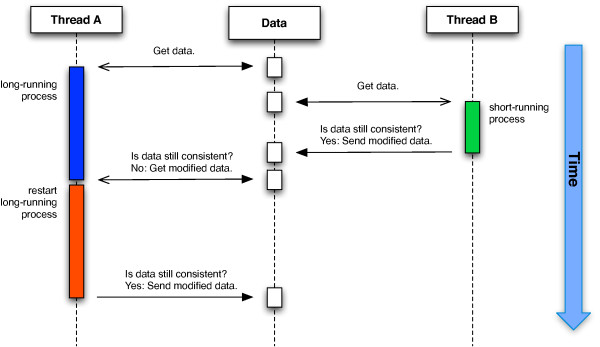
\includegraphics[width=0.7\textwidth]{STM.jpg}
    \caption{Two threads updating shared data~\cite{kestlerBMC}}
    \label{fig:STM.jpg}
\end{figure}

Instead both the threads read the initial state of the data and then go their own ways. They continue to perform their own operations, and when they are ready to commit their changes, they check if the data version has changed since they last read it. 
\begin{itemize}
    \item If it has, they abort their transaction and start over. 
    \item If it hasn't, they can safely commit their changes. 
\end{itemize}

This example shows how lock-less transactional memory can allow both threads to work independently without blocking each other, leading to better performance and scalability.  
\subsection{Haskell}
Haskell has a strong emphasis on immutability and pure functions. This makes it an ideal candidate for STM, as it allows for easier reasoning about concurrent programs.  Haskell is purely functional with a strong type system; most data is immutable, and the side-effects including I/O are tightly controlled by monads~\cite{haskellWiki}. 

\begin{longtable}{|p{0.25\textwidth}|p{0.3\textwidth}|p{0.4\textwidth}|}
    \caption{Summary of design choices for Haskell based on~\cite{harrisComposable,harrisLockFree,harrisTransactional,tankenobuWiki,bartoszBeyondLocks}}
    \label{tab:Haskell-STM Design Choices} \\
    \hline
    \textbf{Design Primitive} & \textbf{Associated Hazards} & \textbf{Reason for Use} \\
    \hline
    \endfirsthead
    \hline
    \textbf{Design Primitive} & \textbf{Associated Hazards} & \textbf{Reason for Use} \\
    \hline
    \endhead
    \hline
    \endfoot
    \hline
    \endlastfoot
    \codeify{TVar} & 
    Memory overhead from versioning; restricted mutation outside transactions &	
    Enables optimistic concurrency control while maintaining type safety. Prevents direct access to shared state outside transactions. \\
    \hline
    \codeify{retry} &
    Indefinite blocking if dependencies never change &
    Automatically restarts transactions only when relevant state changes, avoiding busy waiting. Enabled by dependency tracking via TVar versioning. \\
    \hline
    \codeify{orElse} &
    Increased contention if alternatives access overlapping TVars &	
    Allows composable transaction alternatives without manual coordination. Reduces need for nested exception handling. \\
    \hline
    type-enforced STM/I/O separation &
    Limits expressiveness (no I/O in transactions) &
    Ensures transactions remain rollback-safe. Leverages Haskell's purity to avoid irreversible side effects. \\
    \hline
    optimistic concurrency (no locks) &
    High retry rates under contention &	
    Avoids lock acquisition overhead in common cases. Aligns with Haskell's allocation-heavy workloads where conflicts are rare. \\
    \hline
    per-thread transaction logs &	
    Memory overhead scaling with thread count &	
    Enables lock-free progress guarantee: at least one thread always commits without global synchronization. \\
    \hline
    global version clock &
    Clock overflow risk (64-bit memory address space) &
    Provides a consistent view of shared state across threads. Avoids global synchronization for version updates. \\
    \hline
    phase-fair reader/writer locks &
    Priority inversion in contended writes &
    Ensures progress for both readers and writers. Critical for real-time systems using STM. \\
    \hline
    eager conflict detection &
    False positives in long transactions &
    Minimizes wasted work by aborting early. Complements optimistic approach by failing fast. \\
    \hline
    block-structured heap &
    Memory fragmentation from large objects &
    Enables efficient parallel GC. Allows STM metadata (\codeify{TVar} versions) to coexist with regular objects. \\
    \hline
    cooperative multitasking &
    STM deadlocks in allocation-free loops &
    Avoids OS thread overhead. Mitigated by \codeify{-fomit} yields flag inserting yield points. \\
    \hline
    blackhole-based thunk evaluation &
    Duplicated computation in races &
    Prevents multiple threads evaluating same thunk. Uses CAS for thread-safe lazy evaluation. \\
    \hline
\end{longtable}
This environment mitigates many STM pitfalls like preventing I/O inside transactions (you must use retry or other STM primitives), so the “invisible I/O” problem is solved by the type system. The result is that Haskell STM can offer robust, composable concurrency abstractions (e.g. transactional queues TBQueue, TChan, etc.) with minimal unexpected interactions~\cite{haskellWiki, tankenobuWiki}.


\subsection{Clojure}
Clojure’s entire identity/state model was built with STM in mind. Clojure’s data structures are immutable and persistent, and the only way to have coordinated shared state is via refs in a dosync block. Rich Hickey’s rationale emphasizes “immutable persistent data structures” plus “built-in concurrency support via STM and asynchronous agents”~\cite{hickeyRationale}.

\begin{longtable}{|p{0.25\textwidth}|p{0.3\textwidth}|p{0.4\textwidth}|}
    \caption{Design choices for Clojure based on~\cite{volkmannClojure}} \label{tab:Clojure-STM Design Choices} \\
    \hline
    \textbf{Design Primitive} & \textbf{Associated Hazards} & \textbf{Reason for Use} \\
    \hline
    \endfirsthead
    \hline
    \textbf{Design Primitive} & \textbf{Associated Hazards} & \textbf{Reason for Use} \\
    \hline
    \endhead
    \hline
    \endfoot
    \hline
    \endlastfoot
    \codeify{ref} (Transactional Reference)	&
    Write skew without ensure; version storage overhead	&
    Enables coordinated, atomic updates to multiple shared variables.  
    Uses Multi-Version Concurrency Control (MVCC) for snapshot isolation \\
    \hline
    \codeify{dosync} (Transaction Block) &
    Retry floods under high contention; indefinite blocking if dependencies never change &
    Provides atomicity and isolation for transaction blocks. Uses optimistic concurrency with automatic retries \\
    \hline
    \codeify{alter} (Synchronous Update) &
    Transaction restarts on conflict; potential deadlock if combined with locks &	
    Guarantees sequential consistency by detecting conflicts during commit. \\
    \hline
    \codeify{ensure} (Anti-Write-Skew) &
    Overhead of tracking additional reads &
    Prevents write skew by enforcing read consistency. Required when transactions make decisions based on observed values. \\
    \hline
    \codeify{MVCC} (Multi-Version Concurrency Control) &
    Memory overhead from version history; garbage collection pressure &	
    Allows readers to access consistent snapshots without blocking writers. Critical for Clojure’s immutable data model \\
    \hline
    Fine-Grained Locking (v4/v5) &	
    Deadlock risk if lock order varies; barging prioritization complexity &	
    Enables concurrent commits on disjoint refs. Reduces contention vs global locks. Barging (v5) improves liveness via transaction priorities. \\
    \hline
    Agents for Side Effects &
    Asynchronous execution complicates error handling; \codeify{await} blocking &
    Isolate side effects (I/O) outside transactions. Agents serialize actions per ref, ensuring post-commit execution. \\
    \hline
    Snapshot Isolation &
    ABA scenarios impossible due to versioning &
    Transactions see a consistent snapshot of all refs at the start. Eliminates ABA by tracking version history. \\
    \hline
    \codeify{retry}/\codeify{orElse} &
    Indefinite blocking if dependencies never change &
    \codeify{retry} restarts transactions only when relevant \codeify{refs} change. \codeify{orElse} enables composable decision trees. \\
    \hline
\end{longtable}

In practice though, many Clojure programs end up using simpler primitives like atoms or persistent queues, but the option of STM is always there and shapes how other features work. For instance, atoms (lock-free single-ref updates) only make sense because data is immutable, a design inspired by STM’s snapshot view. Even if Clojure refs aren’t used “99.9\% of the time”, the fact that the language and libraries expect STM means that concurrency is built on a solid foundation of the immutable design, which were designed for STM~\cite{news.ycombinator.com}.

\subsection{Rust}
Rust is a systems programming language that emphasizes safety and performance. It has a strong type system and ownership model, which makes it an ideal candidate for STM. Rust's ownership model ensures that data is either mutable or immutable, which helps to prevent side effects in away that is similar to Haskell. Rust's type system also allows for easy reasoning about concurrent programs, as it enforces strict rules about data access and ownership~\cite{rustWiki}.
\begin{longtable}{|p{0.25\textwidth}|p{0.3\textwidth}|p{0.4\textwidth}|}
    \caption{Design choices for Rust based on~\cite{rustSTM,asyncRustSTM}} \label{tab:Rust-STM Design Choices} \\
    \hline
    \textbf{Design Primitive (library/crate)} & \textbf{Associated Hazards} & \textbf{Reason for Use} \\
    \hline
    \endfirsthead
    \hline
    \textbf{Design Primitive (library/crate)} & \textbf{Associated Hazards} & \textbf{Reason for Use} \\
    \hline
    \endhead
    \hline
    \endfoot
    \hline
    \endlastfoot
    \codeify{TVar<T>} (\codeify{stm},\codeify{async-stm-rs}) & 
    Memory overhead from versioning; garbage collection issue &	
    Enables transactional variables with atomic access. Uses MVCC for snapshot isolation. \\
    \hline
    \codeify{atomically} (\codeify{stm})&
    Retry loops under high contention; indefinite blocking if dependencies never resolve &
    Executes transactions atomically. Pessimistic reads with optimistic commit validation. \\
    \hline
    \codeify{atomically} (\codeify{async-stm-rs})&
    \codeify{tokio} runtime dependency; task cancellation complexity &	
    Non-blocking async transactions for Tokio integration. Allows STM in async contexts without thread starvation. \\
    \hline
    \codeify{retry} (\codeify{stm},\codeify{async-stm-rs} )&
    Livelock if dependencies remain same &
    Aborts or restarts transactions until read \codeify{TVar}s change. Composable via dependency tracking. \\
    \hline
    \codeify{orElse} (\codeify{stm},\codeify{async-stm-rs})&
    Nested transaction overhead; implicit dependency graphs &	
    Provides alternative execution paths if the first transaction retries. Enables decision trees without need for manual coordination.\\
    \hline
    Thread-local transactions (\codeify{async-stm-rs})&	
    Limited to single-threaded async tasks &	
    Simplifies \codeify{TVar} API by passing transactions implicitly via thread-locals. Reduces boilerplate. \\
    \hline
    Hybrid persistent STM (\codeify{async-stm-rs}) &
    Increased complexity for auxiliary transactions &
    Commits/rolls back external state (e.g., databases) alongside STM transactions. Enables consistency across systems. \\
    \hline
\end{longtable}

These features are implemented through external libraries like \codeify{stm}~\cite{rustSTM} and \codeify{async-stm-rs}~\cite{asyncRustSTM}. Former provides STM support for Rust, while the latter async programming support for Rust.\\ 

We also look at design choices of an experimental STM implementation called TORTIS (try-once real-time STM)~\cite{nordTortis}.
It uses a new method for STM called R\textsuperscript{2}STM, which is a hybrid of optimistic and pessimistic concurrency control. It uses a combination of locks and transactions to provide a more efficient and scalable STM implementation. The design choices for TORTIS are as follow:\\
\begin{longtable}{|p{0.25\textwidth}|p{0.3\textwidth}|p{0.4\textwidth}|}
    \caption{Design choices for TORTIS~\cite{nordTortis}} \label{tab:Rust-TORTIS Design Choices} \\
    \hline
    \textbf{Design Primitive} & \textbf{Associated Hazards} & \textbf{Reason for Use} \\
    \hline
    \endfirsthead
    \hline
    \textbf{Design Primitive} & \textbf{Associated Hazards} & \textbf{Reason for Use} \\
    \hline
    \endhead
    \hline
    \endfoot
    \hline
    \endlastfoot
    Retry-free approach (R\textsuperscript{2}STM) & 
    Potentially reduced concurrency and throughput compared to retry-based approaches &	
    Improved scheduling, better bounds on synchronization-related delays, enables I/O within transactions, eliminates the need for retry bounds in worst-case execution time analysis. \\
    \hline
    Lock-based synchronization (on a group of transaction)&
    Traditional lock-based approaches can lead to deadlock &
    Enables retry-free execution, and deadlock is prevented through static analysis and resource grouping\\
    \hline
    \codeify{orElse} &
    Coarse-grained locking may limit runtime concurrency &	
    Prevents deadlock without requiring retries, simplifies synchronization while still allowing non-conflicting transactions to execute concurrently. \\
    \hline
    Transaction placement &
    Deeply embedding transactions may cause non-conflicting transactions to be grouped together &
    Allows programmers to control transaction placement for better resource grouping and concurrency \\
    \hline
\end{longtable}


\subsection{Abandonment}

While STM is a powerful concurrency control mechanism, it is not without its challenges. Some prominent implementations have been abandoned due to various reasons, including performance issues, complexity, and lack of community support :
\begin{enumerate}
    \item \textbf{.NET:}  Microsoft (MS) had an adaptation of STM :  STM.NET, that was pulled by 2010. Joe Duffy (lead researcher for parallelism and concurrency at MS) and colleagues found less or no compelling workloads that needed STM. Duffy notes that their final discouraging verdict: many concurrency apps “enjoyed natural isolation,” and heavy sharing often meant “you were doing something wrong"~\cite{infoq.com}.  In its place, .NET heavily promoted Task Parallel Library (TPL), PLINQ for data parallelism, \codeify{async}/\codeify{await} for async I/O, and concurrent collections as simpler models.
    \item \textbf{Python:}  Standard CPython(C-based Interpreter) still has a Global Interpreter Lock (GIL), so technically only one thread executes Python bytecode at a time, thereby limiting true parallelism. Efforts like an experimental STM-based PyPy which uses RPython (R-based Interpreter), attempted to remove the GIL by wrapping every Python bytecode in transactions.~\cite{pypy.org}. This allowed multiple threads to run atomic blocks concurrently, rolling back on conflicts. The approach proved complex and was not adopted to mainstream; instead multiprocessing, asyncio/event loops, and external libraries like Celery took over.
    \item \textbf{Akka:} Around the same time as .NET abandonment, Akka also abandoned its STM implementation.Akka used the Multiverse library and Clojure-style refs for advanced use cases~\cite{docs.akka.io}. 
    However, Akka is fundamentally about the actor model, where each actor has private state and interacts by message passing, unlike STM’s shared-memory transactions. Akka tech lead Roland Kuhn noted that STM was “considered a failed experiment” in their context and “never compatible with distributed computing”~\cite{groups.google.com}.
\end{enumerate}
